\documentclass[class=article, crop=false]{standalone}
\usepackage{my_preamble}
\begin{document}
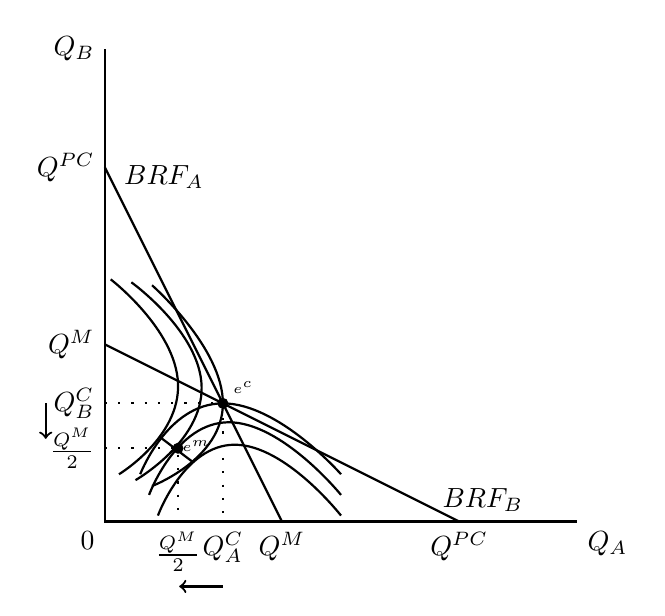
\begin{tikzpicture}[thick,font=\sffamily,scale=1.5]
	%axis
	 \draw (0,4) node[left]{$Q_{B}$} -- (0,0) node[below left] {$0$} -- (4,0) node[below right]{$Q_{A}$};
	  
	 %BRFs
	\draw[] (0,3) -- (1.5,0); %BRF A
	\draw[] (0,1.5) -- (3,0); %BRF B

	%Iso-profits
	\draw[] plot [smooth, tension=1] coordinates {(0.3,0.4) (1,1) (2,0.4)}; %A's iso-profit 1
	\draw[] plot [smooth, tension=1] coordinates {(0.45,0.05) (1.1,0.65) (2,0.05)}; %A's iso-profit 2
	\draw[] plot [smooth, tension=1] coordinates {(0.4,0.3) (1,1) (0.4,2)}; %B's iso-profit 1
	\draw[] plot [smooth, tension=1] coordinates {(0.12,0.4) (0.62,1.17) (0.05,2.05)}; %B's iso-profit 2
	
	%collusion
	\draw[] (0.46,0.72) -- (0.75,0.5); %Contract curve	
	\draw[] plot [smooth, tension=1] coordinates {(0.375,0.225) (1.05,0.84) (2,0.225)}; %A's iso-profit collusion
	\draw[] plot [smooth, tension=1] coordinates {(0.26,0.35) (0.82,1.14) (0.225,2.025)}; %B's iso-profit collusion
	
	%labels
	\node[below] at (0.5,3.1) {$BRF_{A}$}; %BRF A label
	\node[above] at (3.2,0) {$BRF_{B}$}; %BRF B label
	\node[below] at (1.5,0) {$Q^{M}$}; %A's monopoly quantity
	\node[left] at (0,1.5) {$Q^{M}$}; %B's monopoly quantity
	\node[below] at (3,0) {$Q^{PC}$}; %PC quantity - A's???
	\node[left] at (0,3) {$Q^{PC}$}; %PC quantity
	
	%equilibria labels
	\node[style={fill=black,circle,inner sep=0pt,minimum size=4pt}] at (1,1) { };
	\node[above right]at (1,1) {\tiny{$e^{c}$}};
	\node[style={fill=black,circle,inner sep=0pt,minimum size=4pt}] at (0.62,0.62) { };
	\node[right]at (0.57,0.64) {\tiny{$e^{m}$}};
	
	%dotted lines	
	\draw[loosely dotted] (0,1) node[left]{$Q^{C}_B$} -| node[pos=0.25,below=3mm] {} (1,0) node[below]{$Q^{C}_A$}; %cournot dotted lines
	\draw[loosely dotted] (0,0.62) node[left]{$\frac{Q^{M}}{2}$} -| node[pos=0.25,below=3mm] {} (0.62,0) node[below]{$\frac{Q^{M}}{2}$}; %collusion dotted lines	
	
	%arrows
	\draw [->] (1,-0.55) -- (0.63,-0.55); %x arrow
	\draw [->] (-0.5,1) -- (-0.5,0.7); %y arrow
\end{tikzpicture}
\end{document}